% $Header: /cvsroot/latex-beamer/latex-beamer/solutions/conference-talks/conference-ornate-20min.en.tex,v 1.6 2004/10/07 20:53:08 tantau Exp $

\documentclass{beamer}

% This file is a solution template for:

% - Talk at a conference/colloquium.
% - Talk length is about 20min.
% - Style is ornate.



% Copyright 2004 by Till Tantau <tantau@users.sourceforge.net>.
%
% In principle, this file can be redistributed and/or modified under
% the terms of the GNU Public License, version 2.
%
% However, this file is supposed to be a template to be modified
% for your own needs. For this reason, if you use this file as a
% template and not specifically distribute it as part of a another
% package/program, I grant the extra permission to freely copy and
% modify this file as you see fit and even to delete this copyright
% notice.


\mode<presentation>
{
%  \usetheme{Warsaw}
%  \usetheme{Boadilla}
%  \usetheme{Goettingen}
%  \usetheme{Hannover}
%  \usetheme{Madrid}
%  \usetheme{Marburg}
%  \usetheme{Montpellier}
%  \usetheme{Pittsburgh}
  \usetheme{Hawke}
  % or ...

  \setbeamercovered{transparent}
  % or whatever (possibly just delete it)
}


\usepackage[english]{babel}
% or whatever

\usepackage[latin1]{inputenc}
% or whatever

\usepackage{times}
\usepackage[T1]{fontenc}
% Or whatever. Note that the encoding and the font should match. If T1
% does not look nice, try deleting the line with the fontenc.

\usepackage{multimedia}


%%%%%%
% My Commands
%%%%%%

\newcommand{\ml}{{\sc matlab}}
\newcommand{\bfm}[1]{{\boldsymbol{#1}}}
\newcommand{\bx}{\bfm{x}}
\newcommand{\bb}{\bfm{b}}

%%%%

\title[Lecture 29] % (optional, use only with long paper titles)
{Lecture 29 - QR Factorisation}

% \subtitle
% {Include Only If Paper Has a Subtitle}

\author[I. Hawke] % (optional, use only with lots of authors)
{I.~Hawke}
% - Give the names in the same order as the appear in the paper.
% - Use the \inst{?} command only if the authors have different
%   affiliation.

\institute[University of Southampton] % (optional, but mostly needed)
{
%  \inst{1}%
  School of Mathematics, \\
  University of Southampton, UK
}
% - Use the \inst command only if there are several affiliations.
% - Keep it simple, no one is interested in your street address.

\date[Semester 1] % (optional, should be abbreviation of conference name)
{MATH3018/6141, Semester 1}
% - Either use conference name or its abbreviation.
% - Not really informative to the audience, more for people (including
%   yourself) who are reading the slides online

\subject{Numerical methods}
% This is only inserted into the PDF information catalog. Can be left
% out.



% If you have a file called "university-logo-filename.xxx", where xxx
% is a graphic format that can be processed by latex or pdflatex,
% resp., then you can add a logo as follows:

\pgfdeclareimage[height=0.5cm]{university-logo}{mathematics_7469}
\logo{\pgfuseimage{university-logo}}



% Delete this, if you do not want the table of contents to pop up at
% the beginning of each subsection:
%  \AtBeginSubsection[]
%  {
%    \begin{frame}<beamer>
%      \frametitle{Outline}
%      \tableofcontents[currentsection,currentsubsection]
%    \end{frame}
%  }
\AtBeginSection[]
{
  \begin{frame}<beamer>
    \frametitle{Outline}
    \tableofcontents[currentsection]
  \end{frame}
}


% If you wish to uncover everything in a step-wise fashion, uncomment
% the following command:

%\beamerdefaultoverlayspecification{<+->}


\begin{document}

\begin{frame}
  \titlepage
\end{frame}


\section{\texorpdfstring{$QR$ factorisation}{QR factorisation}}

\subsection{\texorpdfstring{$QR$ factorisation}{QR factorisation}}

\begin{frame}
  \frametitle{The full spectrum of a matrix}

  Our aim is to compute the full spectrum of the square $n \times n$
  matrix $A$; that is, we want to find all its eigenvalues. \pause

  \vspace{1ex}

  Method: transform to a simpler problem that is straightforwardly
  solved. E.g.\ transform $A$ to $B$ with same spectrum, but $B$
  triangular: eigenvalues of a triangular matrix are the diagonal
  coefficients. \pause

  \vspace{1ex}

  Schur's theorem shows that every matrix $A$ has a \emph{similar}
  triangular matrix $B$, but is not useful for finding the matrix in
  practice. \pause

  \vspace{1ex}

  The proof of Schur's theorem made repeated use of \emph{Householder
    reflections}; these are generally useful as we shall see later.

\end{frame}

\begin{frame}
  \frametitle{\texorpdfstring{$QR$ factorisation}{QR factorisation}}

  Another decomposition method for a general (not necessarily square)
  matrix: \emph{orthogonal factorisation}. $A$ written as product of
  matrices, some of which are orthogonal (i.e.\ real -- $Q^{\dagger} =
  Q^T$ -- and unitary, $Q^{-1} = Q^{\dagger} = Q^T$).  \pause

  \vspace{1ex}

  Simplest example: \emph{Householder's} $QR$-factorisation
  \begin{equation*}
    A = Q R,
  \end{equation*}
  with $Q$ unitary, $R$ upper triangular. \pause $A$ and $R$ may be $m
  \times n$ matrices, but $Q$ is always square ($m \times m$). \pause

  \vspace{1ex}

  If $A = QR$ with $Q$ unitary then
  \begin{equation*}
    B = R Q = \left( Q^{\dagger} Q \right) R Q = Q^{\dagger} A Q
  \end{equation*}
  which is similar to $A$.

\end{frame}

\begin{frame}
  \frametitle{Householder's factorisation}

  Need factorisation $A = QR$; or construct unitary $Q$ such that
  \begin{equation*}
    Q^{\dagger} A = R
  \end{equation*}
  where $R$ is upper triangular. \pause

  \vspace{1ex}

  Done by iterative process using \emph{Householder transformations}
  \begin{equation*}
    U_k =
    \begin{pmatrix}
      \text{Id}_{k-1} & 0 \\
      0 & \text{Id}_{m-k+1} - \bfm{u}_k \bfm{u}_k^{\dagger}
    \end{pmatrix}.
  \end{equation*} \pause
  Simple generalization of Householder reflections;
  when $k=1$ it \emph{is} a Householder reflection.

\end{frame}


\begin{frame}
  \frametitle{The iterative process}

  To convert original $A$ into upper triangular matrix $R$, at each
  stage construct matrix rotating $k^{\text{th}}$ column of $A$,
  $\bfm{a}_k$, into $\hat{\bfm{e}}_k$ that is zero in all entries
  $>k$. \pause So
  \begin{align*}
    \bfm{e}_1 = \mu_{1,1} \hat{\bfm{e}_1} & = (\mu_{1,1}, 0, \dots, 0)^T. %\\
%    \hat{\bfm{e}}_2 & = (\mu_{2,1}, \mu_{2,2}, 0, \dots, 0)^T
  \end{align*}
  \pause

  At first stage need a Householder reflection to take $\bfm{a}_1$ to
  (a multiple of) $\bfm{e}_1$. The later stages do not care what
  happens to entries ``above'' the diagonal. So they can be multiplied
  by the identity matrix. \pause Thus at each stage a suitable
  Householder transformation
  \begin{equation*}
    U_k =
    \begin{pmatrix}
      \text{Id}_{k-1} & 0 \\
      0 & \text{Id}_{m-k+1} - \bfm{u}_k \bfm{u}_k^{\dagger}
    \end{pmatrix}
  \end{equation*}
  takes column $\bfm{a}_k$ to ``upper triangular'' column $k$ of the
  new matrix, without altering columns $\bfm{a}_l, \,\, l<k$.

\end{frame}

\begin{frame}
  \frametitle{The rotation}

  At each stage rotate (part of) column $\bfm{a}_k$ into ``lower
  triangular'' column $\hat{\bfm{e}}_k$. This gives the vector
  $\bfm{u}$ for the Householder reflection
  \begin{equation*}
    \bfm{u}_k = \frac{\sqrt{2}}{\| \bfm{a}_k - \beta_k \hat{\bfm{e}}_k \|}
    ( \bfm{a}_k - \beta_k \hat{\bfm{e}}_k ),
  \end{equation*} \pause
  where $\beta_k$ is such that
  $\|\bfm{a}_k\| = \beta_k \|\hat{\bfm{e}}_k\|$, so the reflection is a unitary matrix.

  \begin{overlayarea}{\textwidth}{0.4\textheight}
    \only<3|handout:0>{
    \begin{align*}
      U_1A & \,=
      \left(\text{Id}_{m} - \bfm{u}_1 \bfm{u}_1^{\dagger}\right) A
      \\
      &\, = \left(\begin{array}{c|c}
        \beta_1 & *\\
	\hline
	\boldsymbol{0} & W_{m-1}
      \end{array}\right).
    \end{align*}}

    \only<4|handout:0>{
    \begin{align*}
      U_2U_1A & \,=
      \Bigg(\begin{array}{c c}
	\text{Id}_{1} & 0 \\
	0 & \text{Id}_{m-1} - \bfm{u}_2 \bfm{u}_2^{\dagger}
      \end{array}\Bigg)
      \left(\begin{array}{c|c}
        \beta_1 & *\\
	\hline
	\boldsymbol{0} & W_{m-1}
      \end{array}\right)\\
      &\, = \left(\begin{array}{c c|c}
        \beta_1 & * & *\\
	0 & \beta_2 & *\\
	\hline
	\boldsymbol{0} & \boldsymbol{0} & W_{m-2}
      \end{array}\right).
    \end{align*}}

  \only<5|handout:0>{
    \begin{align*}
      U_3U_2U_1A &\,
      = \left(\begin{array}{c c c|c}
        \beta_1 & * & *& *\\
        0 & \beta_2 & * & *\\
        0 & 0 & \beta_3 & * \\
	\hline
	\boldsymbol{0} & \boldsymbol{0} & \boldsymbol{0} & W_{m-3}
      \end{array}\right).
    \end{align*}}

  \only<6>{
    \begin{align*}
      U_4U_3U_2U_1A &\,
      = \left(\begin{array}{c c c c|c}
        \beta_1 & * & *& *& *\\
        0 & \beta_2 & * & *& *\\
        0 & 0 & \beta_3 & *& * \\
        0 & 0 & 0 & \beta_4 & * \\
	\hline
	\boldsymbol{0} & \boldsymbol{0} & \boldsymbol{0} & \boldsymbol{0} & W_{m-4}
      \end{array}\right).
    \end{align*}}
  \end{overlayarea}


\end{frame}


\begin{frame}
  \frametitle{Consequences}

  The result of applying $k$ Householder transforms is
  \begin{equation*}
    U_k U_{k-1} \dots U_2 U_1 A = \left(
      \begin{array}{c|c}
        J & H \\ \hline 0 & W
      \end{array}\right)
  \end{equation*}
  where $J$ is upper triangular. After $n-1$ transforms we have the
  upper triangular matrix $R$ required. \pause

  \vspace{1ex}

  As each $U_i$ is unitary, the product
  \begin{equation*}
    Q^{\dagger} = U_{n-1} U_{n-2} \dots U_2 U_1
  \end{equation*}
  is unitary, and hence
  \begin{equation*}
    Q = U_1 U_2 \dots U_{n-2} U_{n-1}.
  \end{equation*}

\end{frame}


\section{\texorpdfstring{The $QR$ algorithm of Francis}{The QR
    algorithm of Francis}}


\subsection{\texorpdfstring{The $QR$ algorithm of Francis}{The QR
    algorithm of Francis}}


\begin{frame}
  \frametitle{\texorpdfstring{The $QR$ algorithm of Francis}{The QR
      algorithm of Francis}}

  $QR$ algorithm: iterative process that, in the limit, gives upper
  triangular $A_{\infty}$ similar to $A$. \pause Two steps at each
  iteration:
  \begin{enumerate}
  \item Factorize $A_k$ using Householder's algorithm to get
    \begin{equation*}
      A_k = Q_k R_k.
    \end{equation*}
  \item Compute the next guess $A_{k+1}$ using
    \begin{equation*}
      A_{k+1} = R_k Q_k.
    \end{equation*}
  \end{enumerate} \pause

  From the definition
  \begin{equation*}
    A_{k+1}  = R_k Q_k = Q_k^{\dagger} Q_k R_k Q_k = Q_k^{\dagger} A_k Q_k
  \end{equation*}
  so that all members of the sequence are similar. \pause

  \vspace{1ex}

  Start sequence with $A_1 = A$; iterate sequence to produce a
  triangular matrix.% \pause
  If $A_k$ upper triangular then $Q_k = I$: sequence has converged
  \begin{align*}
    A_{k+1} & = A_k .
  \end{align*}


%   We will not prove that this method actually converges to an upper
%   triangular matrix, but we will rely on it.

\end{frame}

% \begin{frame}
%   \frametitle{\texorpdfstring{The $QR$ algorithm of Francis}{The QR
%       algorithm of Francis}}

%   \begin{enumerate}
%   \item Factorize $A_k$ using Householder's algorithm to get
%     \begin{equation*}
%       A_k = Q_k R_k.
%     \end{equation*}
%   \item Compute the next guess $A_{k+1}$ using
%     \begin{equation*}
%       A_{k+1} = R_k Q_k.
%     \end{equation*}
%   \end{enumerate}

%   This gives the itteration scheme
%   \begin{align*}
%     A_{k+1} & = Q_k^{\dagger} A_k Q_k
%   \end{align*}

%   Clearly if $A_k$ is upper triangular then $Q_k = I$ and our sequence has
%   converged
%   \begin{align*}
%     A_{k+1} & = A_k .
%   \end{align*}


% %   We will not prove that this method actually converges to an upper
% %   triangular matrix, but we will rely on it.

% \end{frame}

\begin{frame}
  \frametitle{Example}

  We apply the $QR$ algorithm to
  \begin{equation*}
    A =
    \begin{pmatrix}
      1 & 2 & 3 \\
      4 & 5 & 6 \\
      7 & 8 & 0
    \end{pmatrix}.
  \end{equation*}
  Start from $A_1 = A$, and at each stage we compute the
  $QR$-factorisation, setting $A_{k+1}  = R_k Q_k$. \pause We find
  \begin{overlayarea}{\textwidth}{0.4\textheight}
    \only<2|handout:0>
    {
      \begin{equation*}
        A =
        \begin{pmatrix}
          1 & 2 & 3 \\
          4 & 5 & 6 \\
          7 & 8 & 0
        \end{pmatrix} \rightarrow
        A_2 =
        \begin{pmatrix}
          8.5909 &  -9.2413  &  3.1659\\
          -4.3423 &  -1.0909 &   1.1078\\
          3.1659  &  1.1078 &  -1.5000
        \end{pmatrix}
      \end{equation*}
    }
    \only<3|handout:0>
    {
      \begin{equation*}
        A =
        \begin{pmatrix}
          1 & 2 & 3 \\
          4 & 5 & 6 \\
          7 & 8 & 0
        \end{pmatrix} \rightarrow
        A_3 =
        \begin{pmatrix}
          12.1434 &  -0.1941 &   2.7400 \\
          3.6616 &  -5.8055 &   1.3022 \\
          0.1341 &  -0.2284 &  -0.3379
        \end{pmatrix}
      \end{equation*}
    }
    \only<4|handout:0>
    {
      \begin{equation*}
        A =
        \begin{pmatrix}
          1 & 2 & 3 \\
          4 & 5 & 6 \\
          7 & 8 & 0
        \end{pmatrix} \rightarrow
        A_4 =
        \begin{pmatrix}
          11.6370 &  -5.3339 &  -3.0770\\
          -1.5849 &  -5.2507 &  -0.6576\\
          0.0041  &  0.0146  & -0.3863
        \end{pmatrix}
      \end{equation*}
    }
    \only<5|handout:0>
    {
      \begin{equation*}
        A =
        \begin{pmatrix}
          1 & 2 & 3 \\
          4 & 5 & 6 \\
          7 & 8 & 0
        \end{pmatrix} \rightarrow
        A_5 =
        \begin{pmatrix}
          12.2535 &  -2.9417 &   2.9725\\
          0.7988  & -5.8653  &  1.0822\\
          0.0001  & -0.0011  & -0.3882
        \end{pmatrix}
      \end{equation*}
    }
    \only<6|handout:0>
    {
      \begin{equation*}
        A =
        \begin{pmatrix}
          1 & 2 & 3 \\
          4 & 5 & 6 \\
          7 & 8 & 0
        \end{pmatrix} \rightarrow
        A_6 =
        \begin{pmatrix}
          12.0378 &  -4.1083 &  -3.0373\\
          -0.3683 &  -5.6494 &  -0.8874\\
          0.0000  &  0.0001  & -0.3884
        \end{pmatrix}
      \end{equation*}
    }
    \only<7>
    {
      \begin{equation*}
        A =
        \begin{pmatrix}
          1 & 2 & 3 \\
          4 & 5 & 6 \\
          7 & 8 & 0
        \end{pmatrix} \rightarrow
        A_7 =
        \begin{pmatrix}
          12.1581 &  -3.5634 &   3.0087 \\
          0.1765  & -5.7697  &  0.9800 \\
          0.0000  & -0.0000  & -0.3884
        \end{pmatrix}
      \end{equation*}
    }
  \end{overlayarea}
\end{frame}

\begin{frame}
  \frametitle{Example: 2}


  \begin{columns}
    \begin{column}{0.35\textwidth}
      The matrix
      \begin{equation*}
        A =
        \begin{pmatrix}
          1 & 2 & 3 \\
          4 & 5 & 6 \\
          7 & 8 & 0
        \end{pmatrix}
      \end{equation*}
      has eigenvalues
      \begin{equation*}
        \left\{
          \begin{array}{c}
            12.1229\\ -5.7345\\ -0.3884
          \end{array}\right. .
      \end{equation*}
      The $QR$ algorithm of Francis converges to all eigenvalues linearly.
    \end{column}
    \begin{column}{0.65\textwidth}
      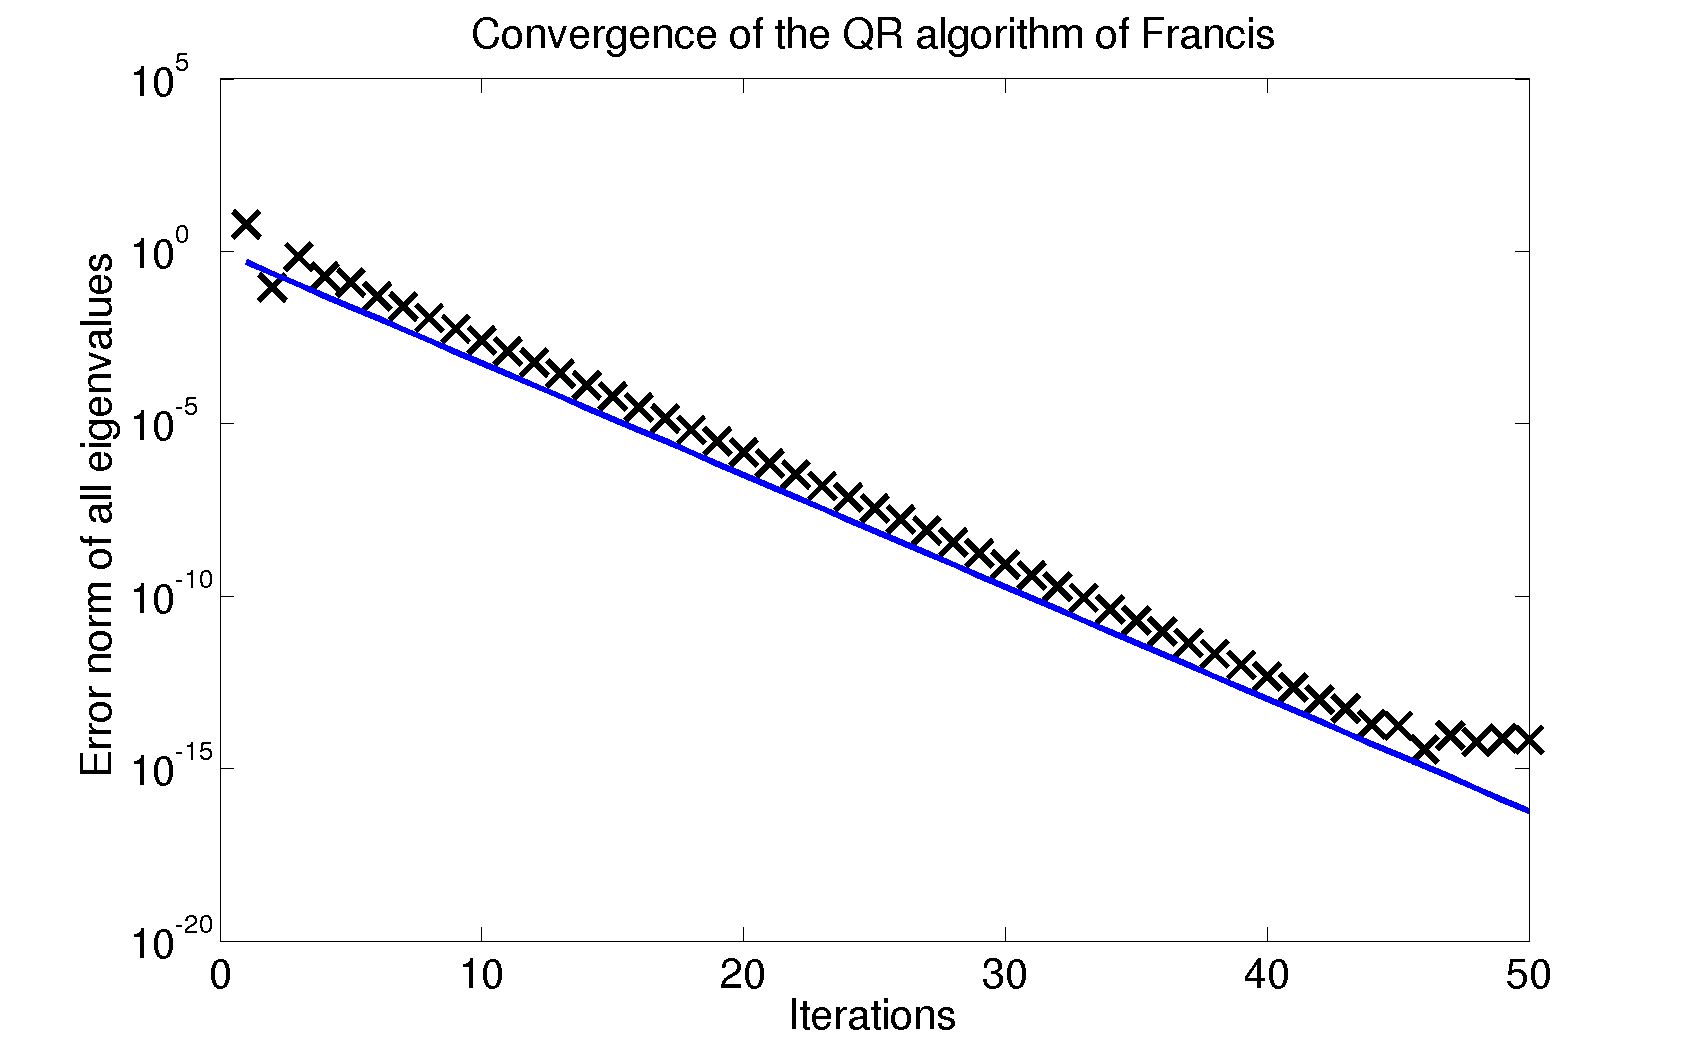
\includegraphics[width=\textwidth]{figures/QRFrancis1}
    \end{column}
  \end{columns}


\end{frame}

\section{\texorpdfstring{$QR$ convergence}{QR convergence}}

\subsection{\texorpdfstring{$QR$ convergence}{QR convergence}}

\begin{frame}
  \frametitle{Comparison with power method}

  Proving that QR algorithm converges not easy. Get some insight from
  comparison with power method.  \pause

  \vspace{1ex}

  Power method: repeated matrix multiplication to find the eigenvector
  of largest eigenvalue.
  %
  \begin{equation*}
    A^k\boldsymbol{x} = \boldsymbol{x}^{(k)} = \lambda_1^k\left[ a_1\boldsymbol{u}_1 +
      \sum_{j=2}^{N}\left(\frac{\lambda_j}{\lambda_1}\right)^ka_j\boldsymbol{u}_j   \right].
  \end{equation*}  \pause
  Obvious extension: apply to multiple vectors
  at the same time.
  \pause

  \vspace{1ex}

  Problem: method will converge to multiple copies of the same
  eigenvector.
\end{frame}

\begin{frame}
  \frametitle{Comparison with power method}

  Overcome problem by \emph{orthonormalising} the vectors at each stage.

  {\centering 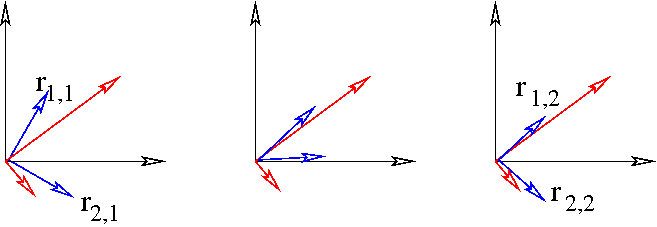
\includegraphics[width=0.8\textwidth]{figures/QR}}
  \pause

  \vspace{1ex}

  $QR$ algorithm does this by expressing the ``guess'' as an
  orthonormal matrix $Q$ at each stage.  \pause

  \vspace{1ex}

  Method works by removing the dominant eigenvector from the
  basis. \pause Remaining ``guesses''  converge to the
  eigenvector of dominant eigenvalue within the resulting subspace.

\end{frame}

\section{Summary}

\subsection{Summary}

\begin{frame}
  \frametitle{Summary}

  \begin{itemize}
  \item To compute all eigenvalues we use the $QR$ algorithm of Francis.
  \item This algorithm is iterative and converges linearly.
  \item It relies on Householder transformations, a generalization of
    Householder reflections.
  \item Each step in the sequence relies on the $QR$ factorisation of
    the matrix. As $Q$ is unitary, each member of the sequence is
    similar and so the spectrum is unchanged.
  \item Interpreting the algorithm as a generalized power method is
    possible but not straightforward.
  \end{itemize}

\end{frame}

\end{document}



%%% Local Variables:
%%% mode: latex
%%% TeX-master: t
%%% End:
